% vim:fileencoding=utf-8:foldmethod=marker:foldmarker=(((,)))

% --- PÁGINA 1: PORTADA ---

\begin{center}

		% === HEADER === (((
		% TITLE
    \vspace*{-0.3cm}
    {\fontsize{26}{28}\selectfont 
    \textbf{El Semillero}\\[-4pt]
    {\fontsize{20}{22}\selectfont \textbf{de}}\\[-3pt]
    \textbf{Grothendieck}\par}
		\vspace{0.4cm}
		% LEMA
		{\large\textit{``Récoltes et semailles''}}
		\vspace{0.5cm}
		% )))

		% === COVER === (((
		\begin{center}
			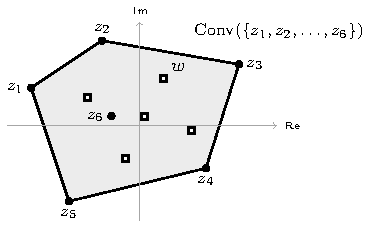
\includegraphics[width= 0.7 \linewidth, page = 1]{pages/01-front-page/images/convex-hull.pdf}
		\end{center}
		\vspace{0.4cm}
		% )))

		% === TABLE OF CONTENTS === (((
		\noindent
		{\footnotesize\bfseries
		\parbox[c]{1.7cm}{\centering\textbf{Esenciales del \\ Estudiante de Licenciatura}}%
		\hfill
		\parbox[c]{1.7cm}{\centering\textbf{Jardín de \\Espacios Topológicos}}%
		\hfill
		\parbox[c]{1.7cm}{\centering\textbf{El Teorema de \\Gauss-Lucas}}%
		\hfill
		\parbox[c]{1.7cm}{\centering\textbf{Matrices Simétricas y\\  Antisimétricas}}%
		}
		\vspace{0.2cm}
		\hrule
		\vspace{0.2cm}
		{\footnotesize Número 1 -- Noviembre 2026}
		% )))

\end{center}

\vspace{0.5cm}
